\question{}

จงศึกษาตัวอย่างโจทย์ต่อไปนี้ แล้วจึงแก้โจทย์ในช่วงท้ายของคำถาม

\marginnote{%
    \centering
    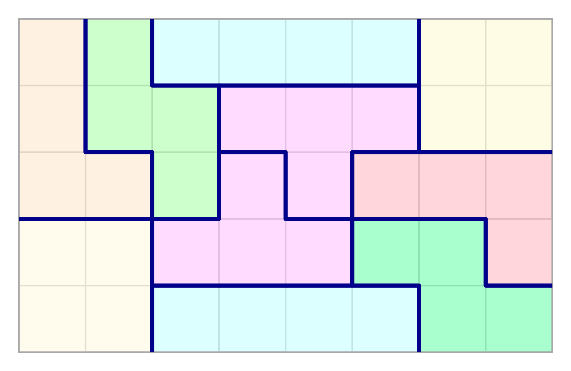
\includegraphics[width=0.98\linewidth]{figures/ponder_national_tetris.eps}
    \vspace{\baselineskip}
}

\smallskip\noindent
\textbf{\uline{ตัวอย่าง}} พิจารณารูปที่ปรากฏทาง\ifpageodd{ขวา}{ซ้าย}มือ 
เป็นพื้นที่สี่เหลี่ยมผืนผ้าขนาด $\mathrm{8 \times 5}$ หน่วย 
ซึ่งถูกตัดแบ่งออกเป็นชิ้นส่วน TETRIS{\textregistered} ประกอบกัน 10 ชิ้น ด้วยการขีดเส้นปากกาดังรูป
(แสดงด้วยเส้นสีน้ำเงินทึบภายในกรอบสี่เหลี่ยม)\; พบว่าความยาวเส้นปากกาดังกล่าวคือ 35 หน่วย\hrsp%
\sidenote{%
    \textbf{หมายเหตุ}\; ความยาวของเส้นปากกา เรานับเฉพาะเส้นที่คั่นระหว่างชิ้นส่วน 
    TETRIS{\textregistered} สองชิ้น และไม่นับเส้นกรอบ
}

สังเกตว่า หากพื้นที่สี่เหลี่ยมผืนผ้านี้ถูกแบ่งเป็นชิ้นส่วน TETRIS{\textregistered} ในรูปแบบที่ต่างออกไป 
อาจจะต้องขีดเส้นปากกาที่มีความยาวรวมมากกว่าหรือน้อยกว่า 35 หน่วยก็ได้

\smallskip\noindent
\textbf{\uline{โจทย์}}\; ให้พิจารณาพื้นที่สี่เหลี่ยมผืนผ้าขนาด $\mathrm{12 \times 9}$ หน่วย 
หากเราใช้ปากกขีดเส้น\uline{ภายใน}
กรอบสี่เหลี่ยม เพื่อแบ่งให้พื้นที่ว่างในกรอบเป็นชิ้นส่วน TETRIS{\textregistered} จำนวน 27 ชิ้น

จงคำนวณหาว่า เส้นปากกาที่ขีดในกรอบสี่เหลี่ยมดังกล่าวจะมีความยาวรวม\uline{น้อยที่สุด}และ
\uline{มากที่สุด}กี่หน่วย?

